 
\documentclass[12pt,twoside]{report}  %twoside, 
\usepackage{abakos}  %pacote com padrão da Abakos baseado no padrão da PUC

%% Comandos de Capa
\newcommand{\monog}{%
\uppercase{TÍTULO DA SUA MONOGRAFIA, DISSERTAÇÃO OU TESE}
}
\title{\monog}
\newcommand{\por}{%
Claudio Davi Souza
}
\author{\por}

\newcommand{\subtitulo}{subtítulo deve começar em letra minúscula}

% Definir macros para o nome da Instituição, da Faculdade, etc.
\newcommand{\univ}{\hspace{0.1cm}Pontifícia \hspace{0.1cm}Universidade\hspace{0.1cm} Católica \hspace{0.1cm}de\hspace{0.2cm} Santa\hspace{0.2cm} Catarina}

\newcommand{\curso}{\hspace{0.1cm} Programa \hspace{0.1cm} de \hspace{0.1cm} Pós-graduação\hspace{0.1cm} em \hspace{0.1cm} Big Data E Data Science}

\newcommand{\grau}{Especialista em Big Data e Data Science }
\newcommand{\tipo}{Monografia}

\newcommand{\profOrientador}{Prof. Nome do Professor}
\newcommand{\profA}{Prof. Nome do Avaliador}
\newcommand{\profB}{Prof. Nome do Avaliador}

\newcommand{\areaConcentracao}{Cadeia de Suprimentos e Previsão de Demanda}

\newcommand{\cidade}{Joinville}

\newcommand{\ano}{2019}

\newcommand{\dataCompleta}{31 de Novembro de 2019}


%%%%%%%%%%%%%%%%%%%%%%%%%%
%Capa da revista
%%%%%%%%%%%%%%%%%%%%%%%%%%

\begin{document}

% %%%%%%%%%%%%%%%%%%%%%%%%%%%%%%%%%% 
% %% Pagina de titulo
% %%%%%%%%%%%%%%%%%%%%%%%%%%%%%%%%%%

\setboolean{@twoside}{false} 
\pagestyle{empty} 
 % \begin{titlepage}
 \singlespace
 \thispagestyle{empty}
 
     \begin{center}
           PONTIFÍCIA UNIVERSIDADE CATÓLICA DE SANTA CATARINA\\
           \curso
     \end{center}
    
    \vspace{3.5cm}
    
    \begin{center}       
         \por     
     \end{center}

     \vspace{3.5cm}
     
     \begin{center}
          \textbf{\monog}\\    %Titulo
          \textbf{\subtitulo}     %Subtitulo          
     \end{center}

      \vfill 
      
      
      \begin{center}
	    \cidade\\
	    \ano
      \end{center}

      \newpage   
   
 \makeatletter
 
% \end{titlepage}


 %%%%%%%%%%%%%%%%%%%%%%%%%%%%%%%%%%%%%
%% Folha de rosto
%% Autor: Fábio Leandro Rodrigues Cordeiro
%% Version: 1.0
%%%%%%%%%%%%%%%%%%%%%%%%%%%%%%%%%%%%%

% Usando o comando \folhaderosto
\setcounter{page}{1}
	\thispagestyle{empty}
  
	\begin{center}
		\por% Autor
	\end{center}
	
	\vfill % Espacamento vertical
	
	\begin{center}
		\textbf{\monog}\\ % Titulo
		\textbf{\subtitulo} % Subtitulo
	\end{center}
	
	\vfill % Espacamento vertical
	
	\begin{flushright}
		\begin{minipage}{9cm} % 7cm (recuo) + 9cm (texto) + 5cm (margens) = 21cm (largura A4)
			 {\tipo apresentada ao \curso~da \univ, como requisito parcial para obtenção do título de \grau.} \par % Nota de apresentacao
			\vspace{1cm}
			Orientador: {\profOrientador} \\ % Orientador 
			Coorientador: {\profA}
			
			\bigskip
			Área de concentração: {\areaConcentracao}

		\end{minipage}
	\end{flushright}
	
	\vfill % Espacamento vertical
	
	\begin{center}
		\cidade\\ % Cidade
		\ano % Ano
	\end{center}
	
	\newpage % Quebra de pagina


% ou...
% fazendo a mao
%
% \begin{titlepage}
%
%   ... codigo da folha de rosto
%  
% \end{titlepage}

 
% %%%%%%%%%%%%%%%%%%%%%%%%%%%%%%%%%%%%%
%% Folha de Aprovação
%% Autor: Maycon Belfort Silva
%% Versão: 1.0
%%%%%%%%%%%%%%%%%%%%%%%%%%%%%%%%%%%%%

%  \begin{folhadeaprovacao}
% \newcommand{\folhaaprovacao}{
\makeatletter	% para usar @

	\thispagestyle{empty}
	
	\begin{center}
		\por % Autor
	\end{center}
	
	\vfill % Espacamento vertical
	
	\begin{center}
		\textbf{\monog}\\ % Titulo
		\textbf{\subtitulo} % Subtitulo
	\end{center}
	
	\vfill % Espacamento vertical
	
	\begin{flushright}
		\begin{minipage}{9cm}
			{\tipo apresentada ao \curso~da \univ, 
			como requisito parcial para obtenção do 
			título  de \grau.} % Nota de apresentacao
			
			\bigskip
			
			Área de concentração: {\areaConcentracao}
			
		\end{minipage}
	\end{flushright}
	
	\vfill % Espacamento vertical
	
	\begin{center}
		\rule{8cm}{0.01cm}\\ % Linha horizontal
		\profOrientador (Orientador) -- PUC Minas % Orientador
	\end{center}
	
	\vfill % Espacamento vertical
	
	\begin{center}
		\rule{8cm}{0.01cm}\\  % Linha horizontal
		\profA (Coorientador) -- PUC Minas  % 1o avaliador
	\end{center}
	
	\vfill % Espacamento vertical
	
	\begin{center}
		\rule{8cm}{0.01cm}\\ % Linha horizontal
		\profB -- ETH Zurich % 2o avaliador
	\end{center}
	
	\vfill % Espacamento vertical
	
	\begin{center}
		\cidade, \dataCompleta % Cidade e data completa
	\end{center}
\makeatletter	% para usar @	
	\newpage % Quebra de pagina

 
% %%%%%%%%%%%%%%%%%%%%%%%%%%%%%%%%%%%%%
%% Dedicatoria
%% Autor: Fábio Leandro Rodrigues Cordeiro
%% Versão 1.0
%%%%%%%%%%%%%%%%%%%%%%%%%%%%%%%%%%%%%
% --- DEDICATORIA ---

% \newcommand{\dedicatoria}[1]


\begin{newpage}
	\thispagestyle{empty}
	\setlength{\baselineskip}{1.5\baselineskip} % Espacamento: 1.5
	\begin{flushright}
	
		\begin{minipage}{12cm} 
		\vspace{15cm}		
		\textit{Dedicatória: Página onde o autor presta homenagem a uma ou mais pessoas.
                        	O layout desta página fica a critério do autor, mas o tipo e tamanho de letras são definidos pela ABNT.}
		\end{minipage}
	\end{flushright}
\end{newpage}

\clearpage
 
 %\begin{newpage}
	\thispagestyle{empty}	
	\setlength{\parindent}{1.25cm} % Paragrafo
	\setlength{\baselineskip}{1.5\baselineskip} % Espacamento: 1.5
	\begin{center}
		\textbf{AGRADECIMENTOS} \\ [1.5\baselineskip]
	\end{center}
	
Agradecimentos a pessoas, instituições ou entidades as quais contribuíram ou ajudaram com  desenvolvimento do trabalho.

\end{newpage} 
 
 %%%%%%%%%%%%%%%%%%%%%%%%%%%%%%%%%%%%%%
%% Epigrafe
%% Autor: Maycon Belfort Silva
%% Versão: 1.0
%%%%%%%%%%%%%%%%%%%%%%%%%%%%%%%%%%%%%


% \pretextualchapter{}

\vspace{7.5cm}
\thispagestyle{empty}
\begin{citacaodireta}

\textit{Pensamentos retirados de livros, músicas, poemas, relacionados ao tema do trabalho.
	Deve ser elaborada conforme norma NBR 10520/2002. Apresentação de citações em documentos.
	Se desejar, a epígrafe pode ser grafada em itálico.
	Ao final do trabalho deve-se fazer a referência. 
	\\
	``Standing on a hill in my mountain of dreams. Telling myself it's not as hard, hard, hard as it seems''} \cite{musica} 
	
\end{citacaodireta}


 % %%%%%%%%%%%%%%%%%%%%%%%%%%%%%%%%%%%%%
%% Resumo
%% Autor: Fábio Leandro Rodrigues Cordeiro
%% Version: 1.0
%%%%%%%%%%%%%%%%%%%%%%%%%%%%%%%%%%%%%

\begin{newpage}
	\thispagestyle{empty}
	\setlength{\baselineskip}{1.5\baselineskip} % Espacamento: 1.5
	\begin{center}
		\textbf{RESUMO} \\ [1.5\baselineskip]
	\end{center}
	\singlespace
	\noindent 
	O resumo deverá conter pelo menos cento e cinquenta palavras de acordo com o padrão de normalização da ABNT. Este artigo abordará as quatro mais importantes linguagens de programação WEB usadas atualmente, comparando suas características de maneira a indicar o melhor uso  de uma linguagem. 
	As linguagens apresentadas serão divididas de acordo com as seguintes características: interpretadas, compiladas, \textit{server-side} e \textit{client-side}. O resumo deverá conter pelo menos cento e cinquenta palavras de acordo com as normas da ABNT.
	linguagens serão divididas de acordo com principais características: interpretadas, compiladas, \textit{server-side} e \textit{cliente-side}. 
	O resumo deverá conter pelo menos cento e cinquenta palavras de acordo com o padrão de normalização da ABNT.
        \vspace{1.5\baselineskip} 
	\par
        \noindent Palavras-chave: {Modelo \LaTeX. Dissertação, Teses. Monografias.}% Palavras-chave
\end{newpage}


{
\begin{newpage}
	\thispagestyle{empty}
	\setlength{\baselineskip}{1.5\baselineskip} % Espacamento: 1.5
	\begin{center}
		\textbf{ABSTRACT} \\ [1.5\baselineskip]
	\end{center}
	\singlespace
	\noindent 
	The abstract should contain at least one hundred and fifty words in accordance with the ABNT standard. This article will address the main features of the web programming 
	languages, more used, comparing their features to indicate the better use of a language. The language will be divided according with four characteristics: 
	interpreted, compiled, server-side and client-side. This article will address the main features of the programming languages. The abstract should contain at least one hundred 
	and fifty words in accordance with the standards of ABNT standard. The language will be divided according with four major characteristics: interpreted, compiled, server-side 
	and client-side. This present article will address the main features of the web programming languages. The abstract should contain at least one hundred and fifty words in 
	accordance with the standards of ABNT standard
        \vspace{1.5\baselineskip} 
	\par
        \noindent Keysords: {Template \LaTeX. Masthertesys. PhD thesys.}
\end{newpage}
}
	
 % %%%%%%%%%%%%%%%%%%%%%%%%%%%%%%%%%%%%%
%% Abstract
%% Autor: Fábio Leandro Rodrigues Cordeiro
%% Version: 1.0
%%%%%%%%%%%%%%%%%%%%%%%%%%%%%%%%%%%%%

\begin{abstract}

This work aim to make a comparative study between two network environments, a single-processor and load divided so they 
can check the behavior of these models in a real situation that is the process of image restoration laboratory at PUC Minas 
from the tool a hard disk cloning. Were first were investigated to define the tools and parameters load testing environments. 
The second step was the preparation of environments, the single-processor with a dedicated server and the cluster of computers that 
had four seasons with the same settings of the client stations.
The third phase of this study was to task the submission of two environmental tests under the same conditions 
generating analytical data, which were used for the last phase of analysis and conclusion of these data. In the last step, 
was identified restrictions on the installation of the solution in a distributed environment with common network, however it 
was noted that this environment is behaving so as to provide load balancing even in the case of large amount of traffic, 
which did not occur in the environment single-processor
\noindent Palavras-chave: {Trivial Database Cluster, Distributed File Systems, Linux}% Palavras-chave

\end{abstract}

	
%tabelas de conteúdo

% \listafiguras
%\listatabelas
% \listaquadros
% \listagraficos 
%\listadesiglas
\addtocontents{toc}{\protect\setcounter{tocdepth}{5}} %para começar a colocar itens no sumário
\setcounter{secnumdepth}{4} %número de hierarquia de seções
\sumario  % \tableofcontents
\setboolean{@twoside}{true} 

%%%%%%%%%%%%%%%%%%%%%%%%%%%%%%%%%%%%%%%%%%%%%%%%%
%% INICIO DO TEXTO
%%%%%%%%%%%%%%%%%%%%%%%%%%%%%%%%%%%%%%%%%%%%%%%%%

%%% Capitulos %%%%
\thispagestyle{myheadings}

\chapter{INTRODUÇÃO}


O sucesso de uma indústria pode ser calculado a partir dos KPIs (\textit{Key Performance Indicator}) desenvolvidos pela mesma. Porém diferente de muitos outros setores, a industria tem poucos KPIs relacionados à cadeia de suprimentos e mesmo os existentes não são difundidos dentre as mesmas. Pouco se sabe sobre processos e criação de KPIs diretamente relacionados à cadeia de suprimentos nas industrias situadas em paises em desenvolvimento \cite{chae2009developing}.

Um dos problemas da industria alimentícia, principalmente a de produtos perecíveis, é como calcular a quantidade de cada SKU (\textit{Stock Keeping Unit}) a ser fabricada nos próximos meses; já que o estoque,  além de capital parado, corre o risco de não chegar às prateleiras do comércio. Quando este chega, tem seu tempo de prateleira significantemente reduzido. Em contrapartida, fabricar produtos abaixo da demanda do mercado leva a perda de receita \cite{aburto2007improved}, Portanto um balanço deve ser atingido.

Visto que um pedido de matéria prima - sendo ele superior à demanda do mercado para o mesmo período -  feita à um fornecedor pode trazer prejuízos para uma industria, todo seu planejamento deve ser cuidadosamente calculado para evitar disperdícios, assim como o planejamento do fornecedor e de toda a cadeia afetada. Dessa forma, grupo de empresas pode se tornar interdependente por ser afetado pelas decisões daqueles que fazem parte da mesma cadeia.

Grande parte das industrias produtoras de alimento em países em desenvolvimento, ainda utilizam sistemas arcaicos em conjunto com predições intuitivas para projetar sua produção. Quando a demanda é sazonal, é ainda mais dificil de calcular a produção de SKUs, causando as perdas mencionadas anteriormente \cite{yenradee2001demand}. Os problemas supracitados sugerem uma avaliação das técnicas atuais de previsão de demanda visando a perspectiva da industria.

\section{Objetivos}
Este trabalho tem como objetivo avaliar as técnicas atuais de previsão de demanda em uma cadeia de suprimentos com foco na visão da industria produtora, visando auxiliar a industria a gerenciar sua produção futura baseada nas suas vendas.
Os objetivos específicos desse trabalho incluem:
\begin{itemize}
\item{Identificar as técnicas de previsão de demanda recomendads pelo meio acadêmico e utilizadas na industria}
\item{Identificar os dados utilizados para fazer a previsão de demanda.}
\end{itemize}

\section{Organização do Trabalho}
Este trabalho será organizado como descrito a seguir:
\begin{itemize}
\item{O Capítulo \ref{theory} descreve os conceitos de Cadeia de Suprimentos, Calculo de Previsão e Aprendizado de Máquina}
\item{O capitulo \ref{revision} apresenta o mapeamento sistemático da literatura visando obter os trabalhos relacionados a este}
\end{itemize}

\chapter{Fundamentação Teórica}\label{theory}

Neste capítulo, serão explorados os conceitos utilizados nesse trabalho, dentre eles conceitos específicos sobre uma cadeia de suprimentos  e sobre aprendizado de máquina, em específico análise de séries temporais.

\section{Cadeia de Suprimentos}
Segundo \citep{mentzer2001defining} uma cadeia de suprimentos pode ser definida como  a coordenação sistêmica e estratégica  das funções de negócio dentro de uma empresa ou de um grupo de empresas. Estas com o propósito de melhorar o desempenho comercial das partes envolvidas.

Com a definição acima, podemos visualizar a cadeia de suprimentos como um \textit{pipeline} multi direcional, onde o fluxo de informação e de produtos flui entre os membros de uma mesma cadeia. Se torna aqui, importante salientar que não se pode confundir logística com cadeia de suprimentos, ainda segundo \citep{mentzer2001defining} logística é a parte do processo da cadeia de suprimentos que implementa e controla o fluxo de produtos, serviços e informações relacionadas. Portanto, a logística pode ser vista como uma das funções dentro de uma cadeia de suprimentos.

\section{Aprendizado de Maquina}

\subsection{Séries Temporais}


\chapter{Revisão da Literatura} \label{revision}



\section{\esp Inserções de ilustrações}

% Figura
\begin{figure}[ht]
	\centering	
	\caption[\hspace{0.1cm}Grade Computacional.]{Uma Grade Computacional como fonte transparente}
	\vspace{-0.4cm}
	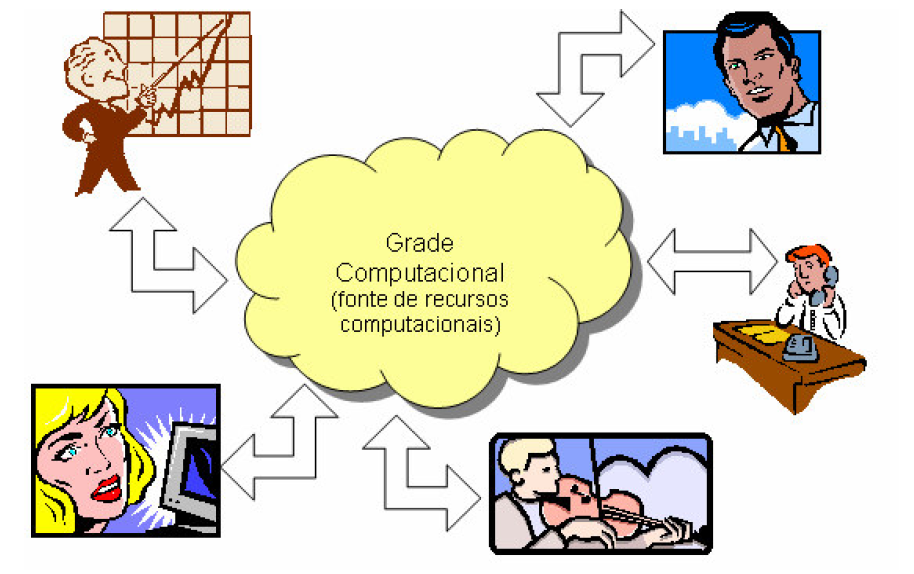
\includegraphics[width=0.6\textwidth]{figuras/grade-comp.png}
	\\\textbf{\footnotesize Fonte: \citeCitacao{cap-livro} }
	\label{fig:figura1}
\end{figure}
\vspace{-0.5cm}

\section{\esp Inserção de tela de software}

% Figura
\begin{figure}[!ht]
	\centering	
	\caption[\hspace{0.1cm}Exemplo de tela de software.]{Exemplo de tela de software}
	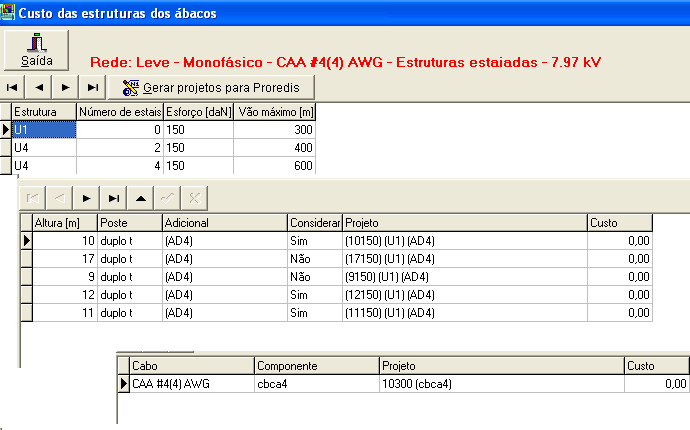
\includegraphics[width=.8\textwidth]{figuras/tela1.png}
	\\\textbf{\footnotesize Fonte: \citeCitacao{tela1}}
	\label{fig:tela1}
\end{figure}

\section{\esp Inserção de gráficos e mapas}

\begin{grafico}
	\centering	
	\graficos{Exemplo de um gráfico}
	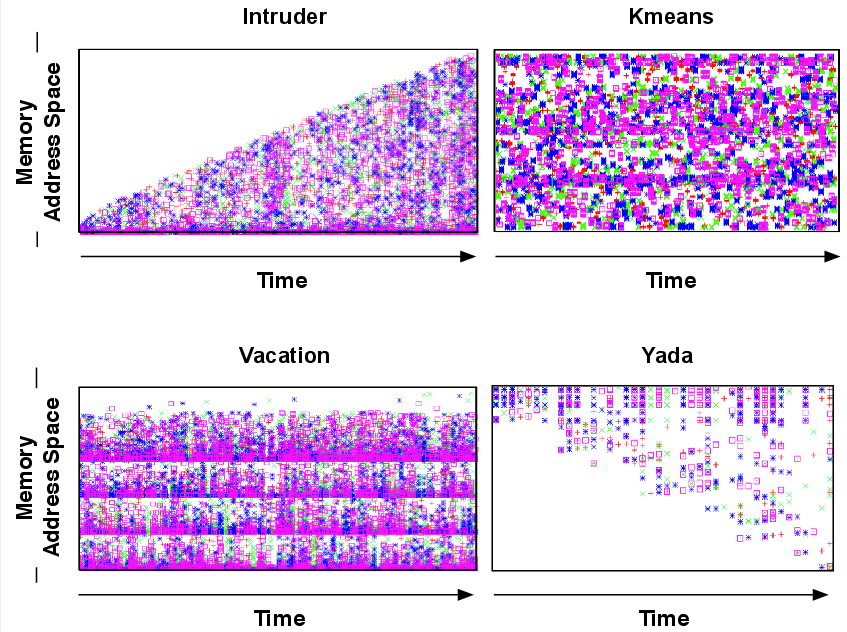
\includegraphics[width=0.7\textwidth]{figuras/access.png}
	\\\textbf{\footnotesize Fonte: \citeCitacao{tese}}
	\label{gra:grafico1}
\end{grafico}


 \section{\esp Tabelas}

% Tabela
\begin{table}[htb]
	\centering
	\caption{\hspace{0.1cm} Exemplo de uma tabela}
	\vspace{-0.3cm} % espaço entre titulo e tabela
	\label{tab:tabela1}
	% Conteúdo da tabela
	\begin{tabular}{l|c|c}
  \hline
    \textbf{Imagem}	& \textbf{transferência} & \textbf{tempo} \\
    \hline
     estação 1	& 7,72 MB/s &  1:22:18 \\
     estação 2	& 7,72 MB/s &  1:22:17 \\
     estação 3	& 7,59 MB/s & 1:24:25 \\
     estação 4  & 7,53 MB/s & 1:43:27 \\
     estação 5	& 6,14 MB/s  &  1:24:41 \\
     estação 6  &  7,50 MB/s & 1:23:53 \\
     estação 7  & 7,58 MB/s  &  1:24:02 \\
     estação 8  & 7,8 MB/s  &  1:29:06 \\
     estação 9  & 7,9 MB/s  &  1:30:05 \\
     estação 10 & 8,0 MB/s  &  1:32:03 \\
     \hline
 \end{tabular}
	\small
	{\footnotesize\\ \textbf{Fonte: \citeCitacao{monog-fabio}}}
\end{table}


\section{\esp Inserção de algoritmos}

\begin{algoritmo}
	\footnotesize
	\algoritmos{Algoritmo genético simples}
	\label{alg:ag}
    \begin{algorithmic}[1]
    		\State Inicialize as probabilidades de cruzamento e mutação, e tamanho da população.
		\State Gere população inicial
		\While{critério convergência não alcançado}
			\State Avalie os indivíduos da população
			\State Execute a seleção
			\State Execute cruzamento
			\State Execute mutação
		\EndWhile{}
  	\end{algorithmic}
	\textbf{\small{Fonte: Adaptado de~\citeCitacao{mestrado}.}}
\end{algoritmo}

\chapter{ CITAÇÕES}


Referências deverão ser adicionadas no arquivo \textit{bibliografia.bib}. Cada referência deverá ser adicionada conforme o padrão de normalização da PUC, 
o qual poderá ser consultado na página da biblioteca da PUC Minas \cite{manualpuc}. Todas as publicações citadas no texto deverão ter correspondente nas referências, 
e as indicações de autoria da citação e do ano deverão ser idênticas aos dados expostos.


\section{\esp Citação livre ou indireta}

Quando se reproduzir ideias, sem transcrever as palavras do autor, a indicação da página é opcional. Exemplos desse tipo de citação:
\begin{enumerate} 
 \item [a)] Citação com um autor \cite{knuth}. 
 \item [b)] Citação de artigos em revistas com dois autores \cite{artigo01}.
  \item [c)] Trabalho em congresso com três autores \cite{dovzan:01}.
 \item [d)] Trabalhos com mais de três autores \cite{cap-livro}.
 \item [e)] Dois autores em duas obras distintas \cite{knuth,groupp}.
 \item [d)] Trabalhos distintos com vários autores \cite{congresso,cap-livro}.
 
\end{enumerate}

\section{\esp Citação direta ou textual}

Transcrição literal de textos de outros autores. Nesse caso, deverão ser especificadas as páginas consultadas. 
Se desejar, poderão ser grafadas em itálico para melhor visualização.

\subsection{\esp Textual Curtas}

Quando curtas (até 3 linhas) serão inseridas na sequência normal do texto, entre aspas com as mesma formatação.

\subsection{\esp Textual Longas}

Citações longas (mais de 3 linhas) deverão constituir um parágrafo independente, recuado a 4 cm da margem esquerda, 
com letra tamanho 10 e digitado em espaço simples, sem aspas.
\begin{citacaodireta}
Hegel chama trabalho à forma específica da satisfação das necessidades, que
distingue da natureza o espírito existente. Assim como a linguagem infringe
a imposição da intuição e ordena o caos das múltiplas sensações em coisas
identificáveis, assim o trabalho infringe a imposição do \hspace{0.1cm}desejo \hspace{0.1cm}imediato \hspace{0.1cm}e
suspende, por assim dizer, o processo de satisfação das necessidades.
\cite[25]{habermas}.
\end{citacaodireta}


% Artigo \cite{whatershed:01}

\subsection{\esp Textual de outros idiomas (Tradução)}

\begin{citacaodireta} 
Um \textit{cluster} é um computador paralelo construído de componentes e processos de \textit{software} (tal como sistema de \textit{software}). 
Um \textit{cluster} é formado de nós, cada um contendo um ou mais processadores, memória que é compartilhada por todos os processadores do nodo 
(somente eles), e dispositivos periféricos adicionais (tais como discos), conectados pela rede e que permitem tráfego de dados entre os nós...
\cite[p. 10, tradução nossa]{groupp}\footnote {  … a cluster is a parallel computer that is constructed of commodity  componets and runs 
(as its system software) commodity software. A cluster is made of nodes, each conteining one or more processors, memory that is  shared 
by all of the processors in (and only on) the node, and addtional peripheral devices (surch as disks),
 connected by network that allows data to move between the nodes}.
\end{citacaodireta}
 
\section{\esp Exemplos de citações} 

Alguns exemplos de citações mais utilizadas e/ou que geram algumas dúvidas. É válido observar que não citaremos
todas as possibilidades de citações da norma da PUC Minas, sendo assim é de extrema relevância que se consulte 
o documento no site da Biblioteca da PUC Minas para maiores esclarecimentos acerca de citações \cite{manualpuc}.

\subsection{\esp Citação de monografia, dissertação e tese}

Exemplo de citação de monografia de curso de graduação ou especialização pode ser vista em \citeonline{monog-fabio}.
Exemplo de dissertação de mestrado é referida como \citeonline{mestrado}.

Para o caso de doutorado é citado da seguinte forma, Góes (\citeyear{tese}). Nesse exemplo é válido observar a forma
como está escrito no documento \LaTeX, pois citações que compreendem no texto o nome do autor como sua parte, necessitam 
do parâmetro \verb$\citeonline{}$. 

\subsection{\esp Livros e partes de livros}

Exemplo de capítulo de livro fica conforme este exemplo \cite{cap-livro}.

Para livros citados no corpo do texto e com duas citações juntas, ver os exemplos \citeonline{knuth,groupp}.
Caso essa citação não fizesse parte do texto será referencia dessa forma \cite{knuth,groupp}.

Citações institucionais ou documentos técnicos de alguma entidade devem ser citados desta forma \cite{pmbok}.

\subsection{\esp Tela de software}

Para  citar a tela de um \textit{software} faça da seguinte forma, \citeonline{tela1}.

\subsection{\esp Citações da Biblia Sagrada}

A Bíblia está dividida em duas grandes partes: O Antigo Testamento e o Novo Testamento, divididos em livros, capítulos e versículos. 
Portanto, a citação de partes da Bíblia deve apresentar o título do livro de forma abreviada ou por extenso, o número do capítulo e o número do versículo.


\begin{citacaodireta}
Moisés estendeu a mão sobre o mar. Com um forte \hspace{-0.1cm} vento \hspace{0.1cm} leste a \hspace{0.1cm}sobrar a
noite toda, o Senhor repeliu o mar e o pôs a seco. As águas se fenderam e
os filhos de Israel entraram no meio do mar a pé enxuto, enquanto as águas
formavam uma muralha à direita e à esquerda deles (\citeauthor{biblia} 14,21).
\end{citacaodireta}

\chapter{ CONCLUSÃO}

Discussão dos resultados obtidos na pesquisa. É onde se colocam as observações do autor. 
Poderá também apresentar sugestões de novas linhas de estudo.

A conclusão deve estar de acordo com os objetivos do trabalho.

A conclusão não deve apresentar citações ou interpretações de outros autores.

 \section{\esp Trabalhos futuros}
% 
 Sugestões de estudos posteriores são ser adicionados subseção deste capítulo de conclusão.


% \selectlanguage{brazilian}
%  \onehalfspace  % espaçamento 1.5 entre linhas
%  \setlength{\parindent}{1.25cm}

%% FIM DO TEXTO

%%%%%%%%%%%%%%%%%%%%%%%%%%%%%%%%%%%

% \selectlanguage{brazil}
%%%%%%%%%%%%%%%%%%%%%%%%%%%%%%%%%%%
%% Inicio bibliografia
%%%%%%%%%%%%%%%%%%%%%%%%%%%%%%%%%%%

%IMPORTANTE PARA BIBLIOGRAFIA SIGA A SEGUINTE INSTRUÇÃO, comente e compile e depois volte ao estado anterior e compile novamente sem limpar cache.
       
  %\bibliography{bibliografia} %%% Descomentar esta linha 

  \referencias{bibliografia}    %%% Comentar esta linha

\appendix
   
%%%%%%%%%%%%%%%%%%%%%%%%%%%%%%%%%%%
   
%% \thispagestyle{empty}

\onehalfspacing 


\appendix
\setcounter{page}{87}
% APÊNDICE A – Título

%  \chapter{\hspace{-0.05cm}PÊNDICE  A - Instalação e Configuração do GlusterFS}
\section*{APÊNDICE A - Instalação e Configuração do GlusterFS}

\section*{Requisitos}

Este trabalho foi configurado com as seguintes versões de \textit{software} conforme visto no Quadro \ref{tab:software}.
No entanto recomenda-se essas versões ou superiores.

\section*{Preparação do Ambiente}

Configurar os arquivos de rede que deve ser feito em todos os nodos que receberam o Gluster \textit{Server}.

Configurar os nomes dos \textit{host}, habilitar a rede e rota de acesso externo:

  \noindent{\textbf{\$ sudo vim /etc/sysconfig/network}}

 \noindent{\textit{NETWORKING=yes}}  \\
 \textit{HOSTNAME=node01.ctdb}  \\
 \textit{GATEWAY=10.0.1.250 } \\
 
 Configurar interface primária de rede:
 
 \noindent{\textbf{\$ sudo vim /etc/sysconfig/network-scripts/ifcfg-eth0}}
 
\noindent{\textit{DEVICE="eth0}}" \\
\textit{BOOTPROTO="static"} \\
\textit{HWADDR="08:00:27:39:11:27"} \\
\textit{NM\_CONTROLLED="yes"} \\
\textit{ONBOOT="yes"} \\
\textit{TYPE="Ethernet"} \\
\textit{IPADDR="10.0.1.1"} \\
\textit{NETMASK="255.255.255.0"} \\

Desabilitar o \textit{firewall} padrão das distribuições Linux baseadas em Red Hat. 
Essa configuração não é recomendada para ambientes em produção, sendo necessário que sejam feitas 
as devidas configurações de permissividade no \textit{Firewall} SELinux e no Iptables nesses ambientes.
Como este experimento foi feito de forma controlada e isolada, isso não foi uma precaução 
bastando desativar esses serviços:

Editar o arquivo do SELinux.

\noindent{\textbf{\$vim /etc/sysconfig/selinux}}

\noindent{\textit{SELINUX=disabled}} \\
\textit{SELINUXTYPE=targeted} \\
\textit{SETLOCALDEFS=0} \\

Desabilitar o serviço de Ipables (deve ser feito em todos nodos envolvidos).

\noindent{\textbf{\$sudo /etc/init.d/iptables stop}

Próximo passo é configurar os nodos da rede de forma a permitir que eles se comuniquem por meio de nome e IP, para isso deve se editar o arquivo “/etc/hosts”, 
e indicar o nome das máquinas e IPs, respectivamente. Realizar este procedimento nas quatro estações servidoras do \textit{cluster}.

\noindent{\textbf{\$sudo vim /etc/hosts}}

\noindent{\textit{127.0.0.1  \quad     localhost }} \\
\textit{127.0.1.1  \quad   localhost.localdomain  \quad  localhost} \\
\textit{10.0.1.1   \quad   node01.cluster.local   \quad  node01} \\
\textit{10.0.2.1   \quad   node02.cluster.local   \quad  node02} \\
\textit{10.0.1.3   \quad   node03.cluster.local   \quad	 node03} \\
\textit{10.0.1.4   \quad   node04.cluster.local	  \quad  node04} \\


\section*{Instalação do GlusterFS Server}

Essa etapa requer que as máquinas tenham acesso a internet para que sejam instalados os pacotes bem como baixadas possíveis dependências.

Certificado que elas possuam acesso Web,  habilitar repositórios extras com:

\noindent{\textbf{rpm --import /etc/pki/rpm-gpg/RPM-GPG-KEY*}} \\
\textbf{rpm --import https://fedoraproject.org/static/0608B895.txt}


Atualizar a lista de repositórios e instalar o \textit{wget}, e baixar a última \textit{release}, 
depois deve-se instalar manualmente e atualizar a ordem de prioridade do \textit{Yum}.

\noindent{\textbf{\$ sudo yum update -y}} \\
\textbf{\$ sudo yum install wget -y}


\noindent{\textbf{\$wget http://dl.fedoraproject.org/pub/epel/6/x86\_64/epel-release-6-8.noarch.rpm}} \\
\textbf{\$ sudo rpm -ivh epel-release-6-8.noarch.rpm }
\textbf{\$ sudo yum install yum-priorities}

Alterar o repositório “epel.repo”

\noindent{\textbf{\$ sudo  vim /etc/yum.repos.d/epel.repo}}

\noindent{\textit{[epel]}} \\
\textit{name=Extra Packages for Enterprise Linux 6 - \$basearch} \\
\textit{\#baseurl=http://download.fedoraproject.org/pub/epel/6/\$basearch} \\
\textit{mirrorlist=https://mirrors.fedoraproject.org/metalink?repo=epel-6\&arch=\$basearch} \\ 
\textit{failovermethod=priority} \\
\textit{enabled=1} \\
\textit{priority=10} \\
\textit{gpgcheck=1} \\
\textit{gpgkey=file:///etc/pki/rpm-gpg/RPM-GPG-KEY-EPEL-6}
\textit{[…]} \\

Instalação do GlusterFS \textit{Server} nos servidores:

\noindent{\textbf{\$ sudo yum install glusterfs-server -y}}

Configurar para que ele seja iniciado automaticamente:

\noindent{\textbf{\$ sudo chkconfig --levels 235 glusterd on}}\\
\textbf{\$ sudo /etc/init.d/glusterd start}

\section*{Configuração do GlusterFS Server}

A configuração consiste em adicionar os \textit{peers} que são os nodos pares que hospedaram os \textit{bricks}, 
dos quais serão exportados como unidade de armazenamento mínimos pelos volumes.

Adicionar cada um dos pares no primeiro nodo, e serão adicionados automaticamente nos demais as informações de 
\textit{peers} de todos servidores pelo GlusterFS:

\noindent{\textbf{\$ sudo gluster peer probe node02}} \\
\textbf{\$ sudo gluster peer probe node03} \\
\textbf{\$ sudo gluster peer probe node04} \\

Será retornado mensagem informando que os pares foram adicionados com sucesso. Para fazer fazer a 
checagem das configurações dos \textit{peers} e se eles estão conectados digite:

\noindent{\textbf{\$ gluster peer status}} \\

\begin{figure}[!htp]
\centering
\caption{gluster peer status}
\vspace{-0.3cm}
\includegraphics[width=1\textwidth]{figuras/config/figura1.png}
\footnotesize\\ \textbf{Fonte: \citeonline{centos2014}}
\label{fig:peer}
\end{figure}

Para adicionar cada volume deve ser informado qual o nome do volume, seu tipo, sua maneira 
de transporte e onde estão localizados seus \textit{bricks} físicos, ou seja os diretórios 
que serão exportados dos servidores remotos, que por sua vez devem ser criados antes desse 
procedimento.

Os diretórios devem ser criados em todos os nodos servidores da seguinte forma:

\noindent{\textbf{\$ sudo mkdir -p /dados/replicate}} \\
\textbf{\$  sudo mkdir -p /dados/distribute} \\
\textbf{\$ sudo mkdir -p /dados/stripe}

Depois pode ser realizado a criação dos volumes em apenas um dos nodos, pois a configuração é 
replicada para todos os outros nodos do \textit{cluster}.

\noindent{\textbf{\$ sudo gluster volume create vol-replicate replica 4 transport tcp node01:/storage/\\replicate node02:/storage/replicate node03:/storage/replicate node04:/storage/\\replicate}}

\noindent{\textbf{\$ sudo  gluster volume create vol-distribute transport tcp node01:/storage/distribute   node02:/storage/distribute node03:/storage/distribute node04:/storage/distribute}}

\noindent{\textbf{\$ sudo  gluster volume create vol-stripe stripe 4 transport tcp node01:/storage/stripe node02:/storage/stripe node03:/storage/stripe node04:/storage/stripe}}

Então cada um dos volumes é habilitado para ser reiniciado:

\noindent{\textbf{\$  sudo gluster volume start vol-distribute}} \\
\textbf{\$  sudo gluster volume start vol-replicate }\\
\textbf{\$  sudo gluster volume start vol-stripe}

Para saber se os  volumes estão funcionando corretamente, verificar o status:

 \noindent{\textbf{\$ sudo gluster volume info nome\_do\_volume}}
 
\begin{figure}[!htp]
\centering
\caption{gluster volume info volume-replicate}
\vspace{-0.3cm}
\includegraphics[width=1\textwidth]{figuras/config/figura2.png}
\footnotesize\\ \textbf{Fonte: \citeonline{centos2014}}
\label{fig:replicate}
\end{figure}


 \begin{figure}[!htp]
\centering
\caption{gluster volume info volume-distribute}
\vspace{-0.3cm}
\includegraphics[width=1\textwidth]{figuras/config/figura3.png}
\footnotesize\\ \textbf{Fonte: \citeonline{centos2014}}
\label{fig:distribute}
\end{figure}

 \begin{figure}[!htp]
\centering
\caption{gluster volume info volume-stripe}
\vspace{-0.3cm}
\includegraphics[width=1\textwidth]{figuras/config/figura4.png}
\footnotesize\\ \textbf{Fonte: \citeonline{centos2014}}
\label{fig:stripe}
\end{figure}

\section*{Instalação do GlusterFS Cliente}

Realizar os mesmos procedimentos iniciais da instalação do GlusterFS \textit{Server}, 
adicionar os repositórios e atualizar a lista de pacotes, depois instalar o GlusterFS Cliente.

\noindent{\textbf{\$ sudo yum install glusterfs glusterfs-geo-replication fuse-devel fuse-libs fuse-ntfs-3g}}

\section*{Configuração do GlusterFS Cliente}

A estação cliente deve estar devidamente configurada para enxergar os servidores por nome no arquivos de \textit{hosts}, 
da mesma forma que foi feito nos nodos servidores. Proceda com a montagem manual dos volumes em um ponto de montagem criado localmente:

\noindent{\textbf{\$ sudo mkdir -p /mnt/replicate}}\\
\textbf{\$ sudo mkdir -p /mnt/distribute} \\
\textbf{\$ sudo mkdir -p /mnt/stripe}

Agora faça a montagem manual dos dispositivos, os volumes remotos:

\noindent{\textbf{\$ sudo mount.glusterfs node01:/vol-replicate /mnt/replicate}}\\
\textbf{\$ sudo mount.glusterfs node01:/vol-distribute  /mnt/distribute}\\
\textbf{\$ sudo mount.glusterfs node01:/vol-stripe /mnt/stripe}

ou

\noindent{\textbf{\$ sudo mount -t glusterfs node01:/vol-replicate /mnt/replicate}}\\
\textbf{\$ sudo mount -t glusterfs node01:/vol-distribute  /mnt/distribute}\\
\textbf{\$ sudo mount -t glusterfs node01:/vol-stripe /mnt/stripe}

A conferência se os volumes foram montados devidamente e estão funcionando é feita 
com o comando:

\noindent{\textbf{\$ sudo df -h}}

 \begin{figure}[!htp]
\centering
\caption{sudo df -h}
\includegraphics[width=1\textwidth]{figuras/config/figura5.png}
\footnotesize\\ \textbf{Fonte: \citeonline{centos2014}}
\label{fig:df}
\end{figure}

É importante observar que essa configuração é volátil, e quando a máquina cliente for reiniciada os discos não estarão mais montando. Para que a configuração seja fixa, 
a montagem pode ser adicionada no arquivo “/etc/fstab” para que seja carregada na inicialização do sistema. Abra o arquivo e adicione nele assim:

\noindent{\textbf{\$ sudo vim /etc/fstab}}

\begin{figure}[!htp]
\centering
\caption{/etc/fstab}
\includegraphics[width=1\textwidth]{figuras/config/figura6.png}
\footnotesize\\ \textbf{Fonte: \citeonline{centos2014}}
\label{fig:fsfab}
\end{figure}

\section*{Considerações da instalação e utilização}

A partir dos pontos de montagem na máquina cliente, os volumes passam a ser acessados distribuindo os arquivos pelos \textit{bricks},
de acordo com as características dos volumes associados a eles.
Qualquer serviço de rede que utilize acesso local a um diretório ou mesmo compartilhamento remoto, pode ser direcionado para 
esses diretórios como: bases de dados, servidores Web, servidores de arquivos dentre outros serviços de rede. 



  
                      
\end{document}



